\documentclass{bioinfo}
\copyrightyear{2016} \pubyear{2016}

\access{Advance Access Publication Date: Day Month Year}
\appnotes{Manuscript Category}

\begin{document}
\firstpage{1}

\subtitle{Subject Section}

\title[scater package]{\emph{scater:} pre-processing, quality control, normalisation and visualisation of single-cell RNA-seq data in R}
\author[McCarthy \textit{et~al}.]{Davis J.~McCarthy\,$^{\text{\sfb 1,2,5}*}$, Kieran R.~Campbell\,$^{\text{\sfb 2,4}}$, Aaron T.~L.~Lun\,$^{\text{\sfb 6}}$ and Quin F.~Wills\,$^{\text{\sfb 2,3}}$}
\address{$^{\text{\sf 1}}$European Molecular Biology Laboratory - European Bioinformatics Institute (EMBL-EBI), Hinxton CB10 1SD, Cambridgeshire, UK;\\
$^{\text{\sf 2}}$Wellcome Trust Centre for Human Genetics, University of Oxford,
Oxford, Oxfordshire, UK;\\
$^{\text{\sf 3}}$Weatherall Institute for Molecular Medicine, University of Oxford, Oxford, Oxfordshire, UK;\\
$^{\text{\sf 4}}$Department of Physiology, Anatomy and Genetics, University of Oxford, Oxford, Oxfordshire, UK;\\
$^{\text{\sf 5}}$St Vincent's Institute of Medical Research, 41 Victoria Parade Fitzroy Victoria 3065, Australia; and \\
$^{\text{\sf 6}}$CRUK Cambridge Institute, Robinson Way, Cambridge CB2 0RE,
Cambridgeshire, UK.
% $^{\text{\sf 4}}$Department of Statistics, University of Oxford, Oxford, Oxfordshire, UK;
}

\corresp{$^\ast$To whom correspondence should be addressed.}

\history{Received on XXXXX; revised on XXXXX; accepted on XXXXX}

\editor{Associate Editor: XXXXXXX}

\abstract{\textbf{Motivation:} Single-cell RNA sequencing (scRNA-seq) is increasingly used to study gene expression at the level of individual cells. However, preparing raw sequence data for further analysis is not a straightforward process. Biases, artifacts, and other sources of unwanted variation are present in the data, requiring substantial time and effort to be spent on pre-processing, quality control (QC) and normalisation.\\
\textbf{Results:} We have developed the R/Bioconductor package \emph{scater} to facilitate rigorous pre-processing, quality control, normalisation and visualisation of scRNA-seq data. The package provides a convenient, flexible workflow to process raw sequencing reads into a high-quality expression dataset ready for downstream analysis. \emph{scater} provides a rich suite of plotting tools for single-cell data and a flexible data structure that is compatible with existing tools and can be used as infrastructure for future software development.\\
\textbf{Availability:} The open-source code, along with installation instructions, vignettes and case studies, is available through Bioconductor at
\href{http://bioconductor.org/packages/scater}{http://bioconductor.org/packages/scater}.\\
\textbf{Contact:} \href{davis@ebi.ac.uk}{davis@ebi.ac.uk}\\
\textbf{Supplementary information:} Supplementary data are available at \textit{Bioinformatics} online.}

\maketitle

\section{Introduction}\label{introduction}

Single-cell RNA sequencing (scRNA-seq) describes a broad class of techniques which profile the transcriptomes of individual cells. This provides insights into cellular processes at a resolution that cannot be matched by bulk RNA-seq experiments \citep{Hebenstreit2011-ig,Shalek2013-kf}. With scRNA-seq data, the contributions of different cell types to the expression profile of a heterogeneous population can be explicitly determined. Rare cell types can be interrogated and new cell subpopulations can be discovered. Graduated processes such as development and differentiation can also be studied in greater detail. However, this improvement in resolution comes at the cost of increased technical noise and biases. This means that pre-processing, quality control and normalisation are critical to a rigorous analysis of scRNA-seq data. The increased complexity of the data across hundreds or thousands of cells also requires sophisticated visualisation tools to assist interpretation of the results.

Numerous statistical methods and software tools have been published for scRNA-seq data \citep{Guo2015-wx,Kharchenko2014-rx,Finak2015-rd,Delmans2016-qc,Angerer2015-sw,Kiselev2016-fu,Julia2015-jt,Trapnell2014-gj}. However, all of these assume that quality control and normalisation have already been applied. Fewer methods are available in the literature to perform these basic steps in scRNA-seq data processing \citep{Ilicic2016-dm}. This issue is exacerbated by the diversity of scRNA-seq data sets with respect to the experimental protocol and the biological context of the study, meaning that a single processing pipeline with fixed parameters is unlikely to be universally applicable. Rather, software tools are required that support an interactive approach to analysis. This allows parameters to be fine-tuned for the study at hand in response to any issues diagnosed during data exploration. The provided functionality should also process the data in a statistically rigorous manner and encourage reproducible bioinformatics analyses.

One of the most popular frameworks for interactive analysis is the R programming language, extended for biological data analysis through the Bioconductor project \citep{Huber2015-en}. While Bioconductor packages have been widely used for bulk RNA-seq data, the existing data structures (like the ExpressionSet class) and methods are not sufficient for scRNA-seq data. This is because they do not support data types or processing methods that are specific to single-cell studies (e.g., cell-cell distance matrices for clustering, cell-based quality control). Extensions to the current computational infrastructure are required to add these capabilities for scRNA-seq analyses.

Furthermore, large-scale single-cell studies will contain data types beyond the expression profiles, such as intensity values from fluorescence-activated cell sorting, cell imaging data, and information from epigenetic and targeted genotyping assays. Appropriate data structures and methods are required that can accommodate these rich datasets for integrative analyses of expression and other assay data along with the accompanying metadata.

In addition, current visualisation methods designed for exploratory data analysis of bulk transcriptomic experiments are unsuited to scRNA-seq data sets containing hundreds or thousands of cells. The large size of each dataset also favours methods such as \emph{kallisto} \citep{Bray2016-pj} and \emph{Salmon} \citep{Patro2015-jf} for rapidly quantifying gene expression, and there is a need for new computational infrastructure to process raw scRNA-seq sequence data into a high-quality expression dataset ready for downstream analysis.

% \enlargethispage{12pt}

Here we present \emph{scater}, an open-source R/Bioconductor software package that implements a convenient data structure for representing scRNA-seq data and contains functions for pre-processing, quality control, normalisation and visualisation. The package provides wrapper functions for running \emph{kallisto} and \emph{Salmon} on raw read data and converting their output into gene-level expression values, methods for computing and visualising quality-control metrics for cells and genes, and methods for normalisation and correction of uninteresting covariates. This is done in a single software environment which enables seamless integration with a large number of existing tools for scRNA-seq data analysis in R. The \emph{scater} package provides basic infrastructure upon which customized scRNA-seq analyses can be constructed, and we anticipate the package to be useful across the whole spectrum of users, from experimentalists to computational scientists.\vspace*{-12pt}


\begin{methods}
\section{Methods, Data and Implementation}\label{methods-data-and-implementation}

\subsection{Case study with scRNA-seq data}\label{case-study-with-scrna-seq-data}

The results presented in the main paper and supplementary case study use an unpublished single-cell RNA-seq dataset consisting of 73 cells from two lymphoblast cell lines of two unrelated individuals. Cells were captured, lysed, and cDNA generated using the popular C1 platform from Fluidigm, Inc. (\href{https://www.fluidigm.com/products/c1-system}{www.fluidigm.com/products/c1-system}). The processing of the two cell lines was replicated across two machines, with the nuclei of the two cell lines stained with different dyes before mixing on each machine. Cells were imaged before lysis, with an example image provided together with these data (see Case Study in Supplementary Material). Samples were sequenced with paired-end sequencing using the HiSeq 2500 Sequencing system (Illumina). RNA-seq reads were were mapped to a custom genome reference, consisting of Homo sapiens GRCh37 (primary assembly from \href{ftp://ftp.ensembl.org/pub/release-75/fasta/homo_sapiens/dna/}{ftp://ftp.ensembl.org/pub/release-75/fasta/homo_sapiens/dna/}, last accessed 14/08/2015), Epstein-Barr Virus type 1 (B95-8 strain, Accession NC\_007605.1) and ERCC RNA spike-ins (ThermoFisher).  Reads in fastq format were aligned using TopHat2 v2.0.12 \citep{Kim2013-qb} using Bowtie2 v2.2.3.0 \citep{Langmead2012-yc} as the core-mapping engine (\verb|--mate-inner-dist 190 --mate-std-dev 40 --report-secondary-alignments|) and other default parameters. Potential PCR duplicates were marked with Picard MarkDuplicates v1.92(1464). Reads mapping uniquely to annotated exon features were counted using htseq-count implemented in HTSeq, version 0.6.1p1 \citep{Anders2015-wf}.

Further case studies using \emph{scater} on published data, for example from 3000 mouse cortex cells \citep{Zeisel2015-ab} and 1200 cells from early-development mouse embryos \citep{Scialdone2016-oa} are available at \href{http://dx.doi.org/10.5281/zenodo.59897}{dx.doi.org/10.5281/zenodo.59897}.

% We used these two genomes -
% Human genome GrCh37 (ENSEMBL release 75)
% EBV : Accession NC_007605.1 (also known as EBV B95-8)
% The reference genome was a merged file of Human, EBV and ERCC spike-ins and all reads were aligned with Tophatv2.0.12, duplicates with Picard MarkDuplicates VN:1.92(1464), reads counted with HTSeq-counts v0.6.1p1
% The remaining methods are same as what I shared with Davis when he was writing his methods (also quoted below).

%These are the commands:
%@PG ID:TopHat VN:2.0.12 CL:/usr/local/genetics/bin/tophat2 --mate-inner-dist 100 --mate-std-dev 50 --num-threads 4 --library-type fr-unstranded -o REX/WTCHG_146282_709508_tophat --transcriptome-index=/data/Genomes/BOWTIE2/GRCh37.EBVB95-8wt.ERCC-transcriptome /data/Genomes/BOWTIE2/GRCh37.EBVB95-8wt.ERCC FASTQ/WTCHG_146282_709508_1.fastq.gz FASTQ/WTCHG_146282_709508_2.fastq.gz

%@PG ID:TopHat.1 VN:2.0.12 CL:/usr/local/genetics/bin/tophat2 --mate-inner-dist 100 --mate-std-dev 50 --num-threads 4 --library-type fr-unstranded -o REX/WTCHG_146283_709508_tophat --transcriptome-index=/data/Genomes/BOWTIE2/GRCh37.EBVB95-8wt.ERCC-transcriptome /data/Genomes/BOWTIE2/GRCh37.EBVB95-8wt.ERCC FASTQ/WTCHG_146283_709508_1.fastq.gz FASTQ/WTCHG_146283_709508_2.fastq.gz

%@PG ID:MarkDuplicates PN:MarkDuplicates VN:1.92(1464) CL:net.sf.picard.sam.MarkDuplicates INPUT=[/well/bsg/projects/CP140108/merge/merged_BAM/lol_1_43_accepted_hits_merge.bam] OUTPUT=/well/bsg/projects/CP140108/merge/merged_deDup_BAM/lol_1_43_accepted_hits_merge_deDup.bam METRICS_FILE=/well/bsg/projects/CP140108/merge/merged_deDup_BAM/Metrics/lol_1_43_accepted_hits_merge_deDup.bam.metrics.txt REMOVE_DUPLICATES=true TMP_DIR=[/well/htseq/TMP] VERBOSITY=ERROR    PROGRAM_RECORD_ID=MarkDuplicates PROGRAM_GROUP_NAME=MarkDuplicates ASSUME_SORTED=false MAX_SEQUENCES_FOR_DISK_READ_ENDS_MAP=50000 MAX_FILE_HANDLES_FOR_READ_ENDS_MAP=8000 SORTING_COLLECTION_SIZE_RATIO=0.25 READ_NAME_REGEX=[a-zA-Z0-9]+:[0-9]:([0-9]+):([0-9]+):([0-9]+).* OPTICAL_DUPLICATE_PIXEL_DISTANCE=100 QUIET=false VALIDATION_STRINGENCY=STRICT COMPRESSION_LEVEL=5 MAX_RECORDS_IN_RAM=500000 CREATE_INDEX=false CREATE_MD5_FILE=false


\begin{figure}[!tpb]%figure1
\centerline{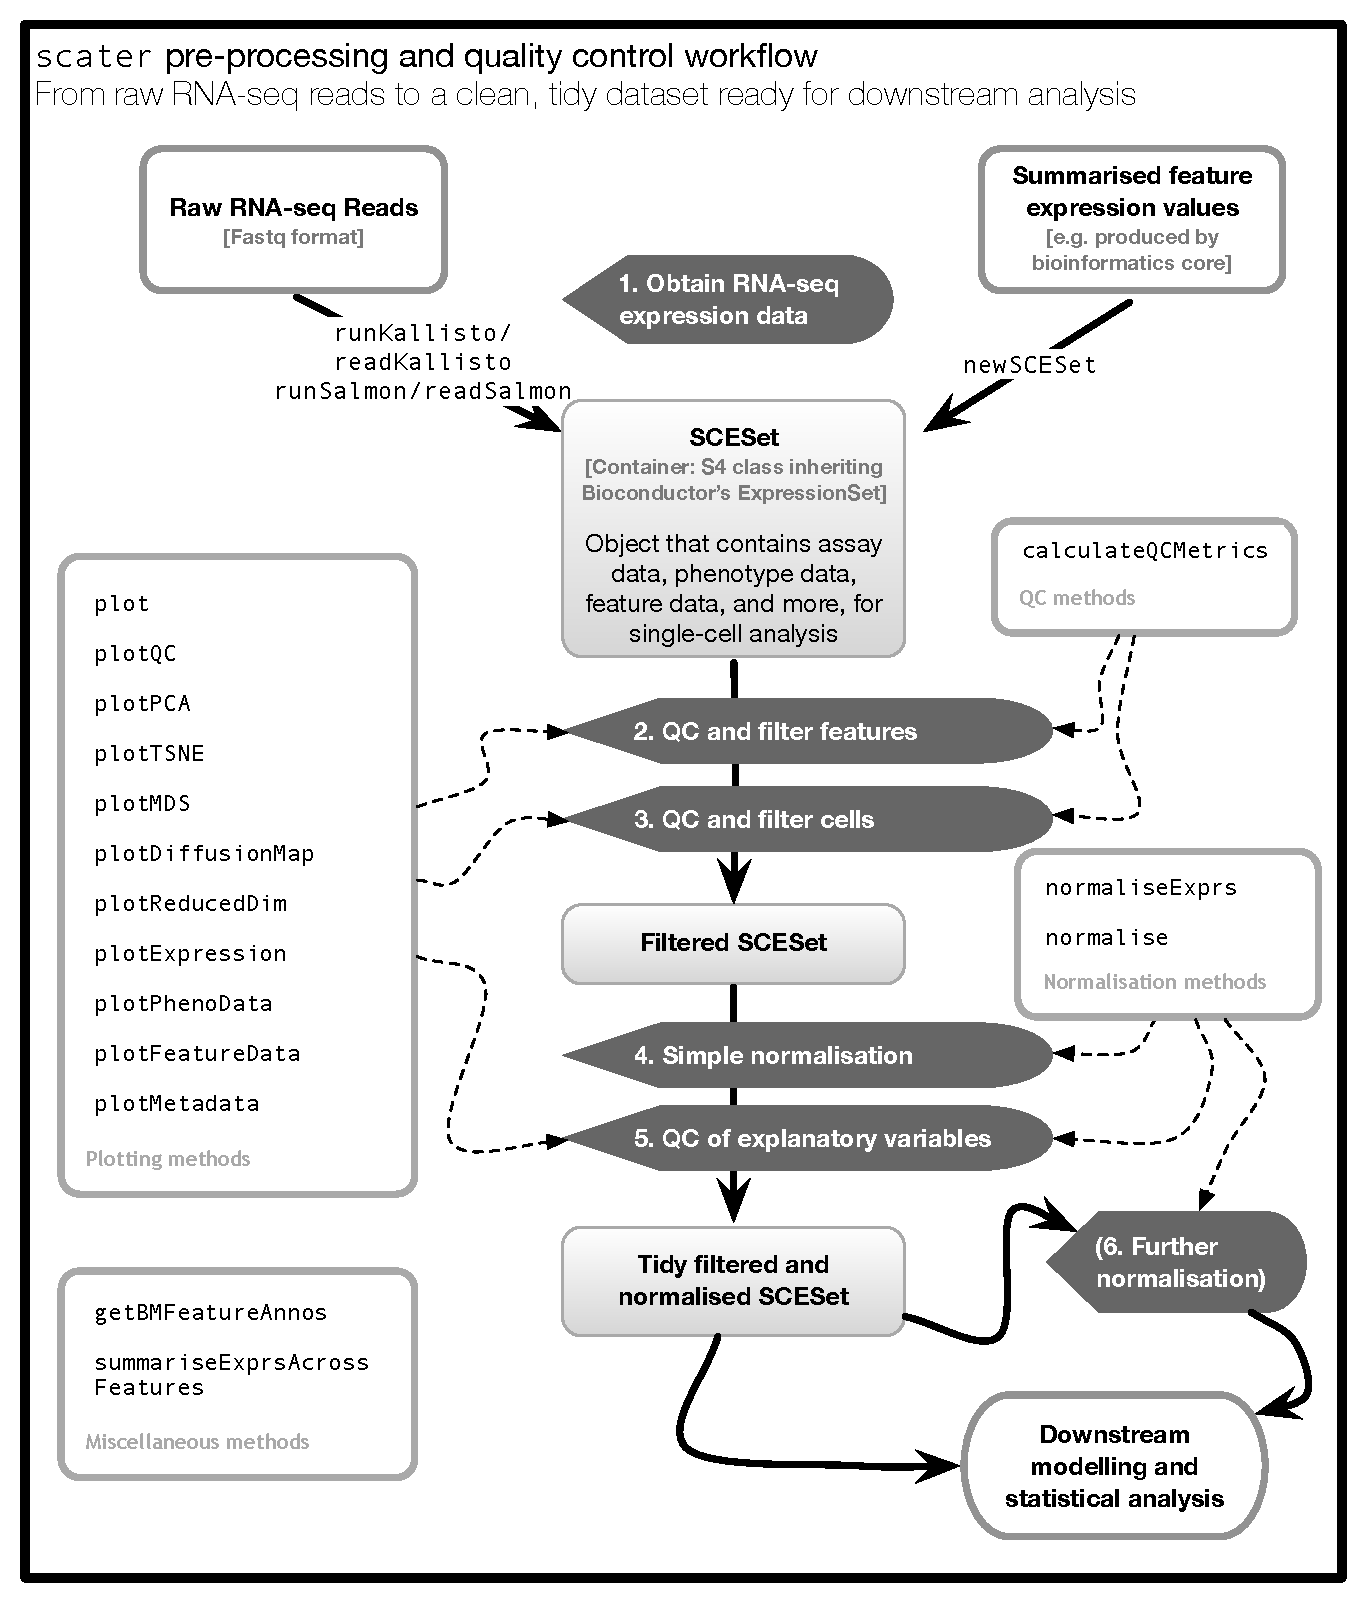
\includegraphics[width=0.48\textwidth]{figures/scater_qc_workflow.pdf}}
\caption{An overview of the \emph{scater} workflow, from raw sequenced reads to a tidy data set ready for higher-level downstream analysis. For step 5, explanatory variables include experimental covariates like batch, cell source and other recorded information, as well as QC metrics computed from the data. Step 6 describes an optional round of normalisation to remove effects of particular explanatory variables from the data. Automated computation of QC metrics and extensive plotting functionality support the workflow.}\label{fig:01}
\end{figure}


\subsection{Implementation}\label{implementation}

The \emph{scater} package is an open-source R package available through     Bioconductor. Key aspects of the code are written in C++ to minimise computational time and memory use. The package builds on many other R packages, including \emph{Biobase} and \emph{BiocGenerics} for core Bioconductor functionality \citep{Huber2015-en}; \emph{destiny} \citep{Angerer2015-sw} and \emph{Rtsne} \citep{Krijthe2015-is} for dimensionality reduction; and \emph{edgeR} \citep{Robinson2010-ky} and \emph{limma} \citep{Ritchie2015-so} for model fitting and statistical analyses. The plotting functionality in the package uses \emph{ggplot2} \citep{Wickham2016-dc}. A full set of dependencies is provided in the Supplementary Materials.

\end{methods}


\section{Results}\label{results}

\subsection{The \emph{scater} package}\label{the-scater-package}

The \emph{scater} package offers a workflow to convert raw read sequences into a data set ready for higher-level analysis within the R programming environment (Figure~\ref{fig:01}). In addition, \emph{scater} provides basic computational infrastructure to standardise and streamline scRNA-seq data analyses. Key features of \emph{scater} include: (1) the ``single-cell expression set'' (SCESet) class, a data structure specialized for scRNA-seq data; (2) wrapper methods to run \emph{kallisto} and \emph{Salmon} and process their output into gene-level expression values; (3) automated calculation of quality control metrics, with QC visualisation and filtering methods to retain high-quality cells and informative features; (4) extensive visualisation capabilities for inspection of scRNA-seq data; and (5) methods to identify and remove uninteresting covariates affecting expression across cells. The package integrates many commonly used tools for scRNA-seq data analysis and provides a foundation on which future methods can be built. The methods in \emph{scater} are agnostic to the form of the input data and are compatible with counts, transcripts-per-million, counts-per-million, FPKM or any other appropriate transformation of the expression values.


\subsection{SCESet: a data structure for single-cell expression
data}\label{sceset-a-data-structure-for-single-cell-expression-data}

The \emph{scater} package is built around the SCESet class (Supplementary Figure~1) which provides a sophisticated container for scRNA-seq data. This class inherits from the ExpressionSet class in Bioconductor's \emph{Biobase} package \citep{Huber2015-en}, which allows assay data (and multiple transformations thereof), gene or transcript metadata and sample metadata to be combined in a single object to empower robust analyses. While the ExpressionSet class is the basis of many microarray and bulk RNA-seq anaysis methods in Bioconductor, extensions to the class design are necessary to support scRNA-seq data analyses. Specifically, the SCESet class adds slots to store a reduced-dimension representation of the expression profiles, to easily visualize the relationships between cells; cell-cell and gene-gene pairwise distance matrices, for clustering or regulatory network reconstruction; bootstrapped expression results (such as from \emph{kallisto}), to gauge the accuracy of expression quantification; consensus clustering results, where cluster assignments for each cell are combined from different methods to improve reliability; information about feature controls (such as ERCC spike-ins), which is required in downstream steps such as normalization, QC and detection of highly variable genes; and several more (Supplementary Figure~1). With these extra slots, SCESet objects can support analyses of scRNA-seq data that ExpressionSet cannot. In addition, extra data types such as FACS marker expression or epigenetic information can be easily stored in each SCESet object for integration with the single-cell expression profiles.

An SCESet data object can be easily subsetted by row or column to remove unwanted genes or cells, respectively, from all data and metadata fields stored in the object. Furthermore, data and metadata in multiple SCESet objects can be easily combined e.g., to incorporate cells from different experimental batches. SCESet objects can also be converted to other R data structures, or saved to disk in structured, shareable formats. Further details on the class, including its motivation and execution, are available in the Supplementary Case Study and the package documentation. All methods available in \emph{scater} are applicable to instances of the SCESet class and exploit the availability and richness of (meta)data stored in each SCESet object.


\subsection{Data pre-processing}\label{data-pre-processing}

An important initial step in scRNA-seq data processing is to quantify the expression level of genomic features such as transcripts or genes from the raw sequencing data. Approaches to expression quantification from raw reads are, in principle, the same for scRNA-seq as they are for bulk RNA-seq \citep{Kanitz2015-wp,Teng2016-sc}. Read counts obtained from conventional quantification methods such as \emph{HTSeq} \citep{Anders2015-wf} and \emph{featureCounts} \citep{Liao2014-ui} can be readily stored in an SCESet object and used in a \emph{scater} workflow (Figure~\ref{fig:01}). Another option is to use computationally-efficient pseudoalignment methods such as \emph{kallisto} and \emph{Salmon}. This is especially appealing for large scRNA-seq data sets containing hundreds to tens of thousands of cells. To this end, \emph{scater} also provides wrapper functions for \emph{kallisto} and \emph{Salmon} so that fast quantification of transcript-level expression can be managed completely within an R programming environment. A common subsequent step for these methods is to collapse transcript-level expression to gene-level expression. Exploiting the \emph{biomaRt} R/Bioconductor package, \emph{scater} provides a convenient function for using Ensembl annotations to obtain
gene-level expression values and gene or transcript annotations \citep{Yates2016-ia}.

\enlargethispage{6pt}

\begin{figure*}[!htpb]%figure3
\centerline{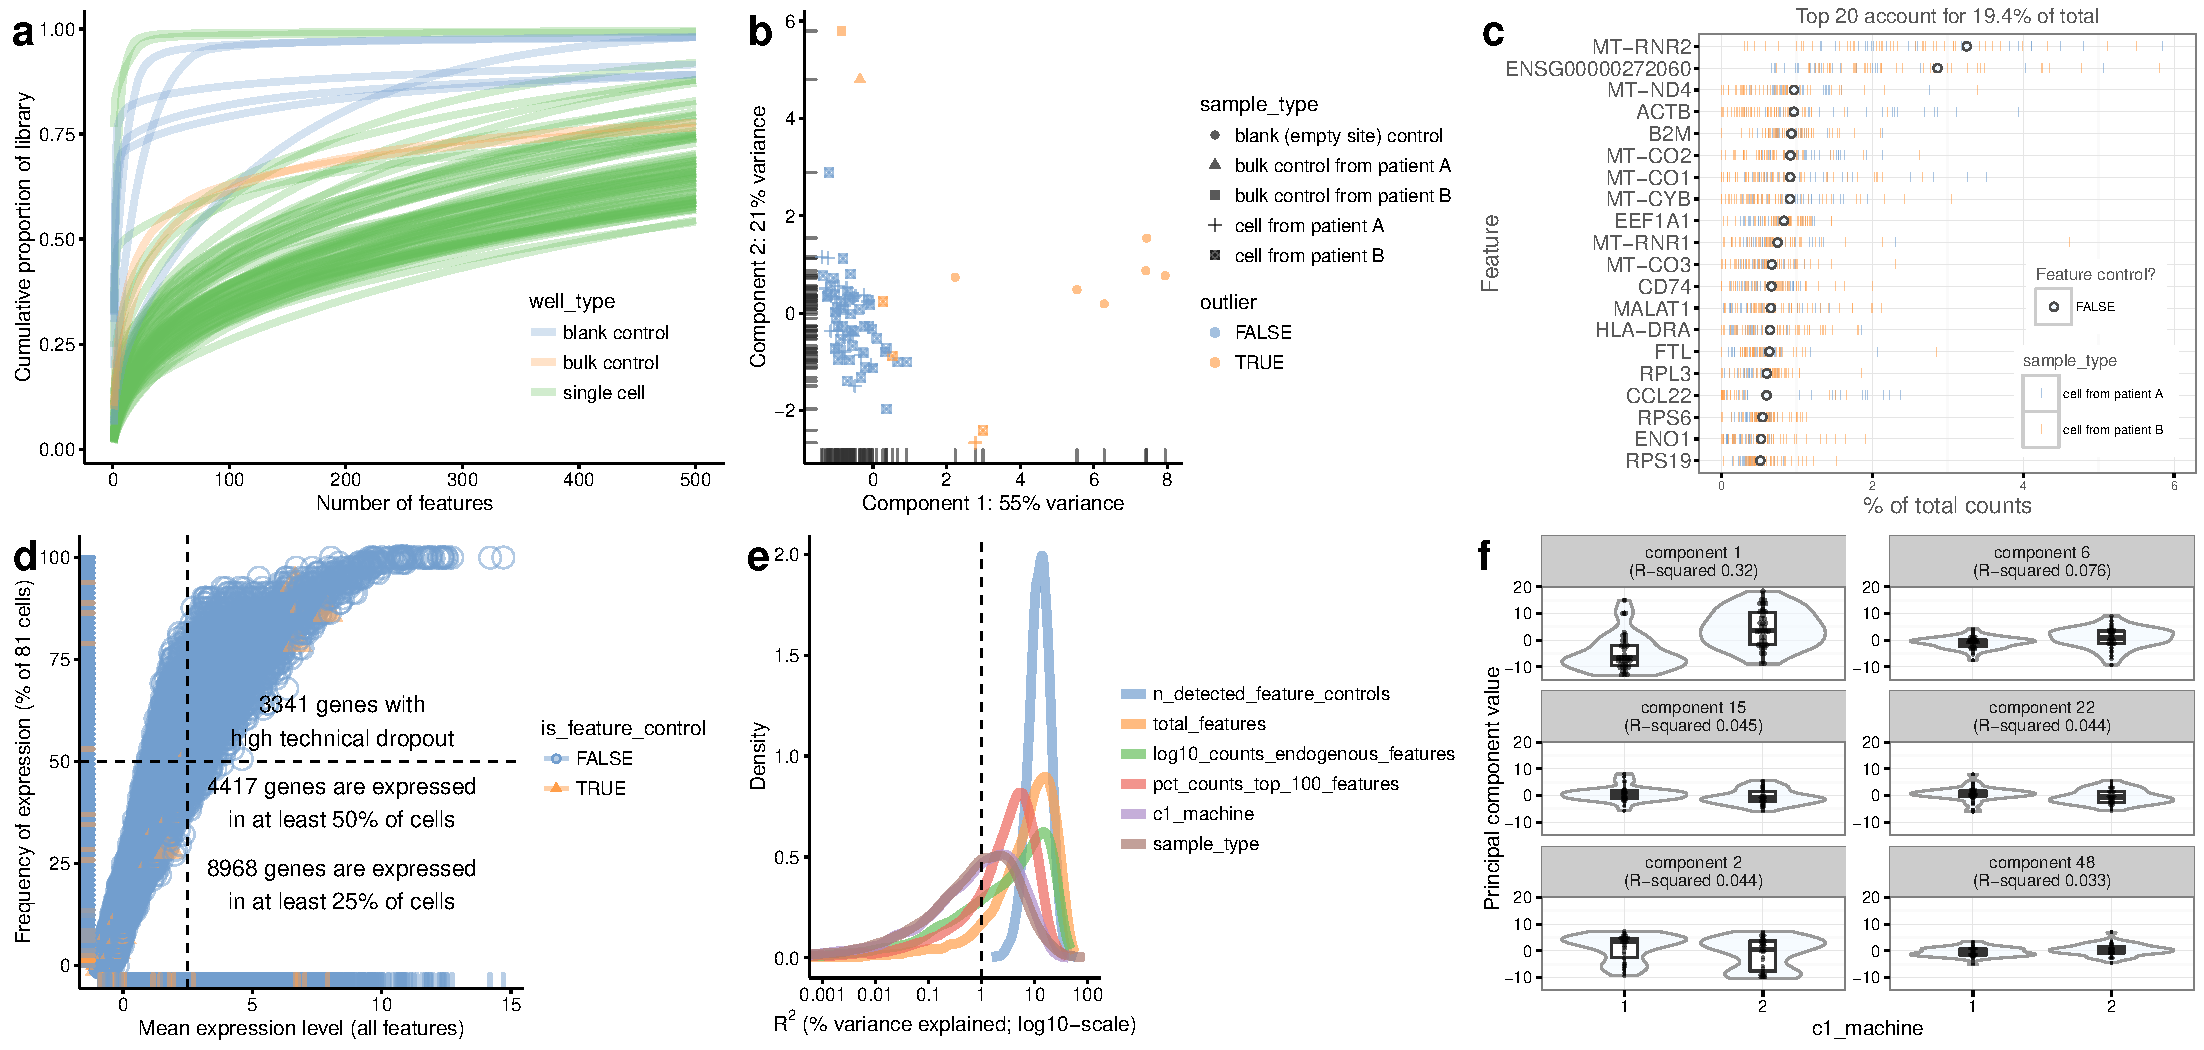
\includegraphics[width=\textwidth]{figures/figure3.pdf}}
\caption{\textbf{Different types of QC plot that can be generated with \emph{scater}.} (\textbf{a}) Cumulative expression plot showing the proportion of the library accounted for by the top 1--500 most highly-expressed features. (\textbf{b)} PCA plot produced using a subset of the QC metrics computed with \emph{scater's} calculateQCMetrics function. (\textbf{c)} Plot of the 50 most-expressed features (computed according to the highest total read counts) across all cells in the data set. For each feature, the circle represents the percentage of counts that the gene accounts for computed from counts pooled across all cells. The genes are ordered by this value. The bars for each gene show the percentage of counts accounted for by the gene for each individual cell, providing a visualisation of the distribution across cells. (\textbf{d}) Plot of frequency of expression (percentage of cells in which the feature is deemed expressed) against mean expression level across cells. (\textbf{e}) Density plot showing the percentage of variance explained by a set of explanatory variables across all genes. (\textbf{f}) Violin, scatter- and boxplots of principal component values against the C1 machine used for each cell for the six principal components most strongly correlated with C1 machine used. Each individual plot is produced by a single call with either the function plot (\textbf{a}), plotPCA (\textbf{b}) or plotQC (\textbf{c-f}).}\label{fig:03}
\end{figure*}


\subsection{Data quality control}\label{data-quality-control}

The \emph{scater} package provides methods to compute relevant QC metrics for an SCESet object. Given a set of control genes and/or cells, a variety of QC metrics will be computed and returned to the object in a single call to the calculateQCMetrics function (see package documentation). Cell-specific QC metrics include the total count across all genes, the total number of expressed genes, and the percentage of counts allocated to control genes like spike-in transcripts or mitochondrial genes. These metrics are useful for identifying low-quality cells---for example, a high percentage of counts mapping to spike-ins typically indicates a small amount of RNA captured for the cell, suggesting protocol failure or death of the cell in processing and means it is unlikely to be suitable for downstream analyses. For each gene, QC metrics such as the average expression level and the proportion of cells in which the gene is expressed are computed. This can be used to identify low-abundance genes or genes with high dropout rates that should be filtered out prior to downstream analyses. All of these metrics are used by scater to construct QC plots to diagnose potential issues with data quality. This facilitates quality control which---despite attempts at automation \citep{Ilicic2016-dm}---still requires manual intervention to account for aspects of the data specific to each study. The package documentation provides full details of the QC metrics produced.

In \emph{scater}, the default plot method for an SCESet object produces
a cumulative expression plot (Figure~\ref{fig:03}a). This plot describes how reads are distributed across genes, distinguishing between low-complexity libraries (where very few genes contain most of the counts) and their high-complexity counterparts (where counts are distributed more evenly across genes).
For example, there is substantial variability in library complexity among cells in the case study dataset in Figure~\ref{fig:03}a. Some cells have profiles similar to the blank wells,
suggesting that library preparation or sequencing failed for these cells and
that the corresponding libraries should be removed prior to further analysis.
Cell phenotype variables can be incorporated into these plots to highlight
differences in expression distributions for different types of cells. For
example, the curve for each cell is coloured by the type of well that produced
the library (Figure~\ref{fig:03}a), while cells can also be split into separate
facets by library type to show more metadata variables simultaneously (see
Supplementary Case Study). Cumulative expression plots should be favoured over
boxplots as the default method for visualising expression distributions across
cells in a dataset, as the latter performs poorly at handling the long tail of
low- and zero-expression observations in scRNA-seq data.

The plotPCA function implements an approach to automatic outlier
detection using multivariate normal methods applied to the cell-level QC
metrics \citep{Ilicic2016-dm}. Specifically, PCA is applied to the QC metrics
for all cells and a plot is produced to automatically detect outliers in the
higher-dimensional QC metric space (Figure~\ref{fig:03}b). These outliers
correspond to low-quality cells with abnormal library characteristics (e.g.,
low total counts and few expressed genes) that should be removed prior to
downstream analysis. This automated approach is powerful but also difficult to interpret, and so complements simpler filtering approaches that apply thresholds to particular QC metrics.

The plotQC function generates many types of plots useful for quality control, such as a plot of visualising the most
highly-expressed features in the dataset (Figure~\ref{fig:03}c). This
provides a feature-centric overview of the dataset that simultaneously
visualises the features with highest total expression across all cells,
while also displaying the distribution of cell-level expression values
for these features. It is common to see ERCC spike-ins (if used),
mitochondrial and ribosomal genes among the highest expressed genes,
while datasets consisting of healthy cells will also show high levels of
constitutively expressed genes like \emph{GAPDH} and \emph{ACTB}. This
plot allows the analyst to quickly check that the gene- or
transcript-level quantification is behaving as expected, and to flag
datasets where it is not.

A key feature of scRNA-seq is the high frequency of ``dropout'' events,
that is, no observed expression (such as no read counts) in a particular
cell for a gene that is actually expressed in that cell. Typically only
a small set of genes are observed with detectable expression in every
cell. The plotQC function can also be used to visualise the frequency of
expression (inverse of the dropout percentage) of features
against their average expression level (Figure~\ref{fig:03}d). Control features
can be highlighted easily in the plot, and typical scRNA-seq datasets will show
a broadly sigmoidal relationship between average expression level and
frequency of expression across cells. This is consistent with expected
behaviour where genes with greater average expression are more readily
captured during library preparation and are detected at a greater
frequency \citep{Brennecke2013-zv,Kim2015-xd,Vallejos2015-ww}.

Another important step in quality control is to identify variables (experimental factors or computed QC metrics) that drive variation in expression data across cells. The plotQC function
provides a novel approach to identifying variables that
have substantial explanatory power for many genes. For each variable in
the phenoData slot of the SCESet object, we fit a linear model for each
feature with just that variable as the explanatory variable. We then plot the distribution of the marginal $R^2$ values across all features for the variables with the most
explanatory power for the dataset (Figure~\ref{fig:03}e). The variables are ranked by median $R^2$ across features in the plot, allowing users to identify variables that may need to be considered
during normalisation or statistical modelling. The plotQC function can
also assess the influence of variables of interest by plotting principal
components of the expression matrix most strongly correlated with a
variable of interest against that variable. For example, in the Case
Study data, the first principal component is correlated with the
C1 machine used to process the cell (Figure~\ref{fig:03}f).

We also introduce the plotPhenoData function for convenient plotting of
cell phenotype information (including QC metrics), and the
plotFeatureData function for plotting feature information (see examples in the
Supplementary Case Study). These methods will work not only on the
SCESet class defined in \emph{scater}, but also on any ExpressionSet object,
providing sophisticated plotting functionality for many other Bioconductor
packages and contexts.

The \emph{scater} graphical user interface (GUI) provides convenient
access to \emph{scater}'s QC and visualisation methods (Supplementary
Figures~3--5). This opens an interactive interface in a web browser that facilitates exploration of the data through QC plots and other intuitive visualisations. The GUI allows users of any background to easily examine the effects of changing multiple parameters, which can be helpful for quickly conducting exploratory data analysis. Useful settings can then be stored in R scripts to ensure that data analyses are reproducible.

In summary, \emph{scater} provides a variety of novel and convenient
methods to visualise an scRNA-seq dataset for QC. Low-quality cells and
uninteresting genes can then be easily removed by filtering and
subsetting the SCESet data structure prior to further analysis.


\subsection{Data visualisation}\label{data-visualisation}

Dimensionality reduction techniques are necessary to convert
high-dimensional expression data into low-dimensional representations
for intuitive visualisation of the relationships, similarities and
differences between cells. To this end, \emph{scater} provides
convenient functions to apply a variety of dimensionality reduction
procedures to the cells in an SCESet object. Functions include plotPCA,
to perform a principal components analysis; plotTSNE, to perform
t-distributed stochastic neighbour embedding \citep{Van_der_Maaten2008-oe}, which has
been widely used for scRNA-seq data \citep{Amir2013-nf,Bendall2014-gf,Macosko2015-vt};
plotDiffusionMap, to generate a diffusion map \citep{Haghverdi2015-fm} for
visualising differentiation processes; and plotMDS, to generate
multi-dimensional scaling plots (Figure~\ref{fig:04}a--c). The plotReducedDim
function can also be used to plot any reduced-dimension representation of cells
(e.g., an independent component analysis produced by \emph{monocle}
\citep{Trapnell2013-fv} or similar) that is stored in an SCESet object.

By default, the PCA and t-SNE plots are produced using the features with
the most variable expression across all cells. We focus on the most variable genes to highlight any
heterogeneity in the data that might be driving interesting differences between
cells. Alternatively, we can apply \emph{a priori} knowledge to define a set of
genes that are associated with a biological process of interest, and construct
plots using only these features. For example, \citealp{Scialdone2015-gj}
found that using prior knowledge to define feature sets is vital for
exploring processes like the cell cycle, which can have substantial effects on
single-cell expression measurements \citep{Buettner2015-jg}. The subsetting
and filtering methods for SCESet objects make it easy to construct
reduced-dimension plots for particular gene sets, in order to
investigate certain effects in the data such as those due to the cell
cycle (Figure~\ref{fig:04}d--f).

The various types of reduced-dimension plots can be used to examine the structure of the cell population, including the formation of distinct subpopulations or the presence of continuous trajectories. Cell-level variables stored in the
SCESet object can be used to define the shape, colour and size of points
plotted, allowing more information to be conveniently incorporated into
each plot (e.g., cells are coloured by \emph{CCND2} expression in
Figure~\ref{fig:04}d--f). The plotExpression function is also provided for
plotting expression levels of a particular gene against any of the cell
phenotype variables or the expression level of
another feature (Figure~\ref{fig:04}g). This allows the user to inspect the expression levels
of a feature or set of features in full detail, rather than relying only
on summary information and reduced-dimension plots where information is
necessarily lost.


\begin{figure}[!tpb]%figure4
\centerline{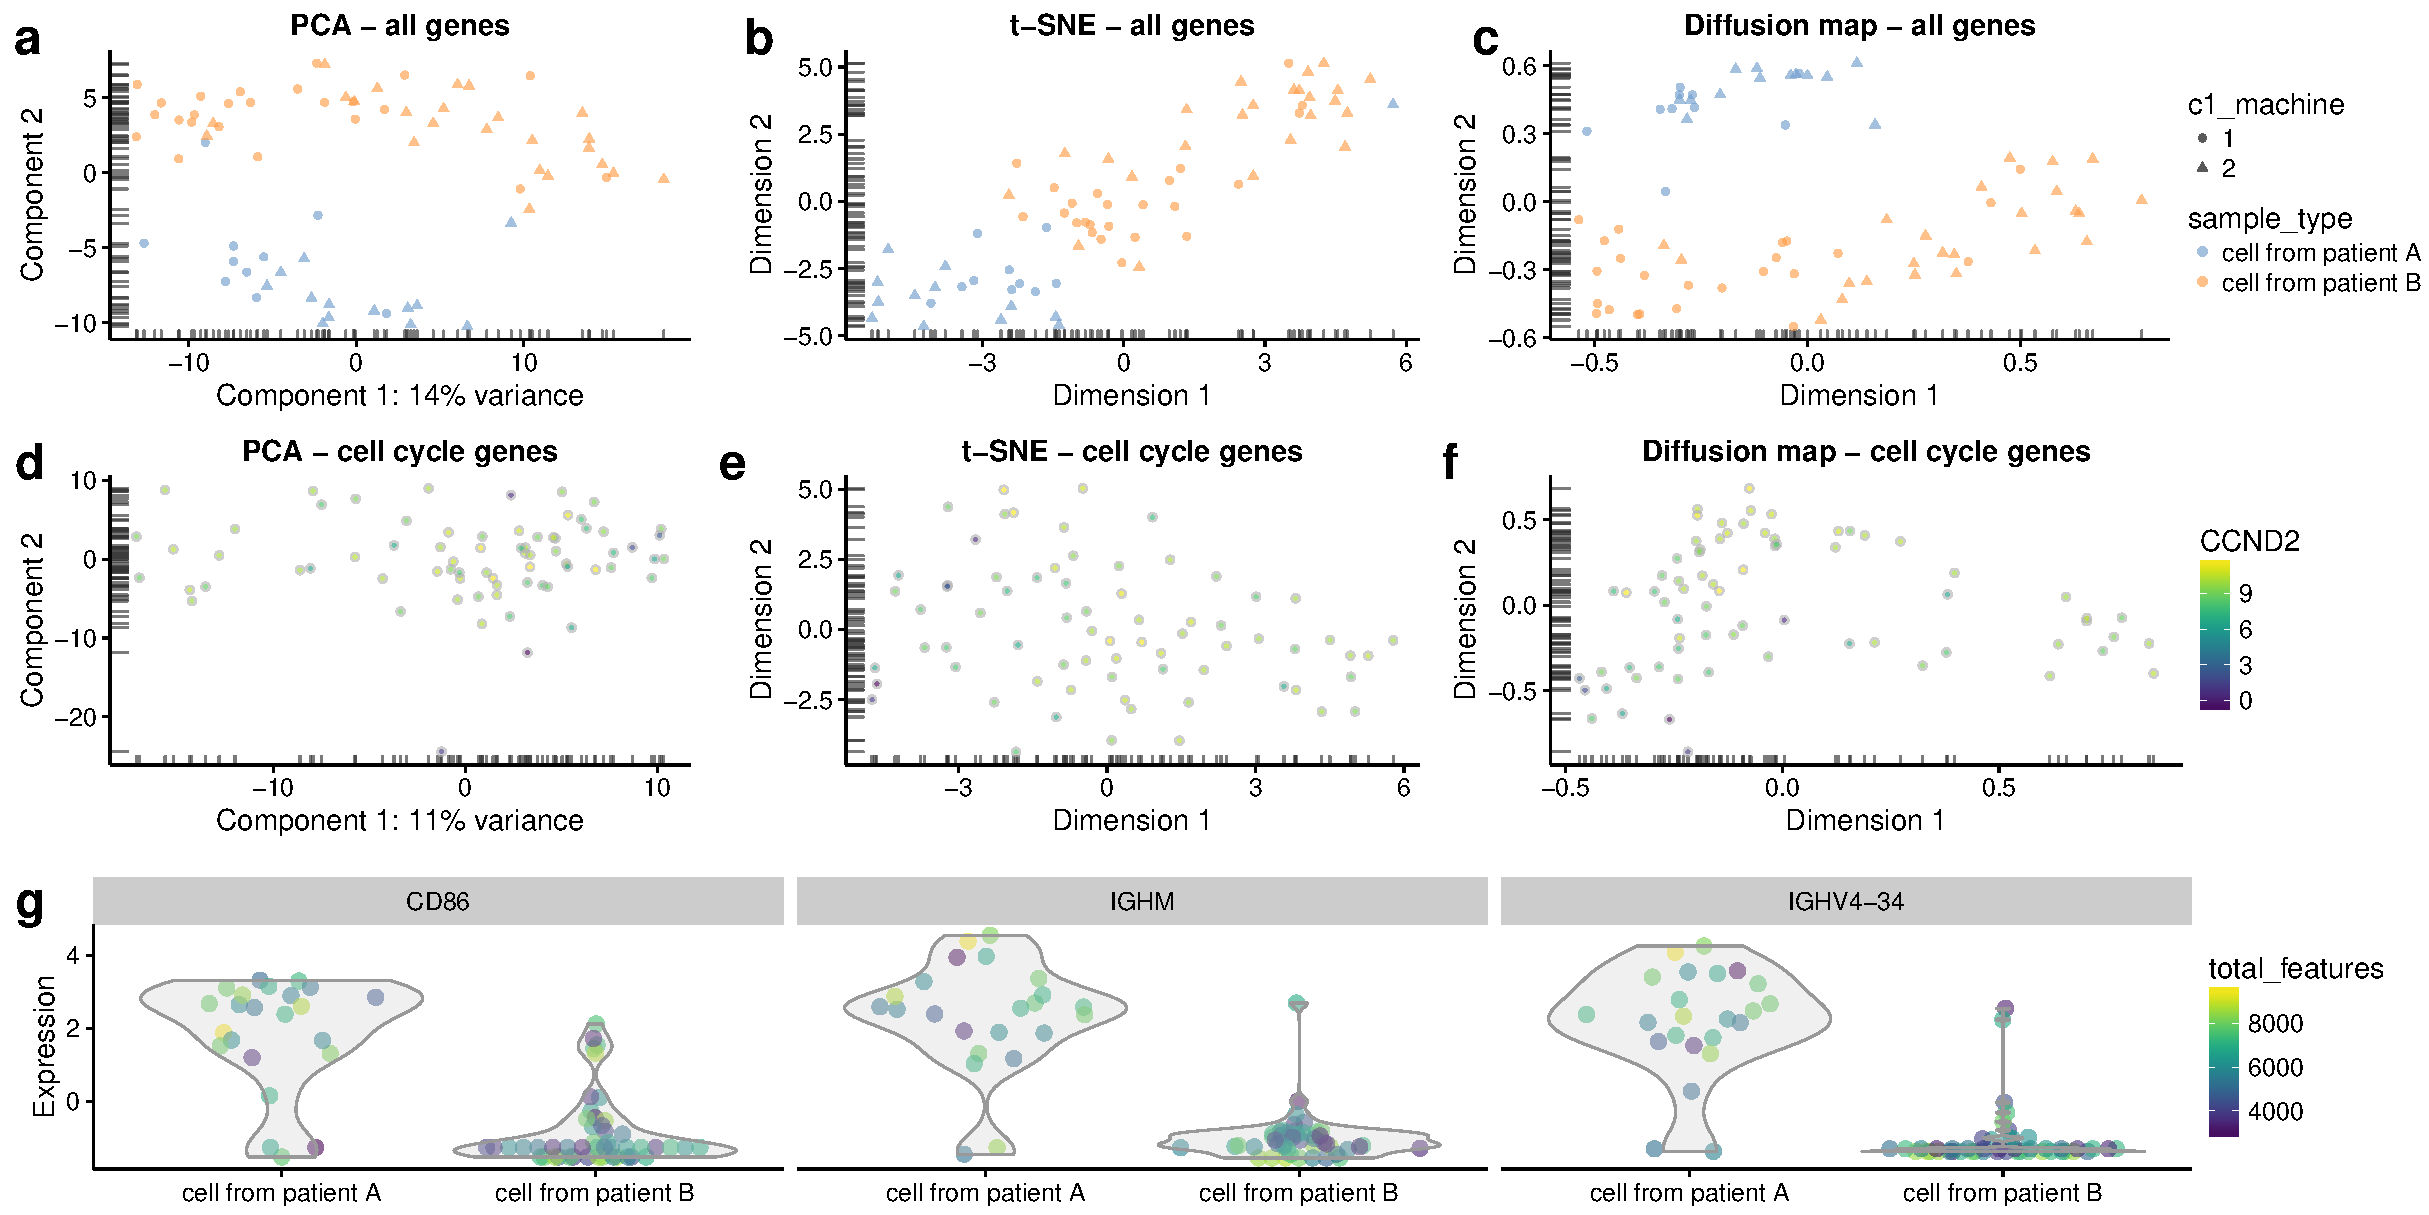
\includegraphics[width=0.48\textwidth]{figures/figure4.pdf}}
\caption{\textbf{Reduced dimension representations of cells and gene expression plots with \emph{scater.}} Plots are shown using all genes (\textbf{a-c}) and cell cycle genes only (\textbf{d-f}) using PCA (\textbf{a,d}), t-SNE (\textbf{b,e}) and diffusion maps (\textbf{c,f}). In the top row (\textbf{a-c}), points are coloured by patient of origin, sized by total features (number of genes with detectable expression) and the shape indicates the C1 machine used to process the cells. In the second row (\textbf{d-f}), points are coloured by the expression of \emph{CCND2} (ENSG00000118971), a gene associated with the G1/S phase transition of the cell cycle. With the plotExpression function, expression for sets of genes can be plotted against any cell metadata variables or the expression of a given gene (\textbf{g}). The function automatically detects whether the x-axis variable is categorical or continuous and plots the data accordingly, with x-axis values ``jittered'' to avoid excessive overplotting of points with the same x coordinate.}\label{fig:04}
\end{figure}


\subsection{Data normalisation and batch correction} \label{data-normalisation-and-batch-correction}

Scaling normalisation is typically required in RNA-seq data analysis to remove biases caused by differences in sequencing depth, capture efficiency or composition effects between samples. Frequently used methods for scaling normalization include the trimmed mean of M-values \citep{Robinson2010-dy}, relative log-expression \citep{Anders2010-kv} and upper-quartile methods \citep{Bullard2010-ui}, all of which are available for use in \emph{scater}. In addition, \emph{scater} is tightly integrated with the \emph{scran} package that implements a method utilising cell pooling and deconvolution to compute size factors better suited to scRNA-seq data \citep{Lun2016-sk}.

After scaling normalisation, further correction is typically required to ameliorate or remove batch effects. For example, in the case study dataset, cells from two patients were each processed on two C1 machines. Although C1 machine is not one of the most important explanatory variables on a per-gene level (Figure~\ref{fig:03}e), this factor is correlated with the first principal component of the log-expression data (Figure~\ref{fig:03}f). This effect cannot be removed by scaling normalisation methods, which target cell-specific biases and are not sufficient for removing large-scale batch effects that vary on a gene-by-gene basis (Figure~\ref{fig:05}a). Here we present two possibilities, all easily implemented in a scater workflow.

The C1 machine effect is known from the design of the experiment, so we
can easily regress out this effect in \emph{scater}. With the
normaliseExprs function the user can supply a design matrix of variables
to regress out of the expression values, and residuals from the linear
model fit can be used as expression values for downstream analyses. For
the dataset here, we fit a linear model to the \emph{scran} normalised
log-expression values with the C1 machine as an explanatory factor. (We
also use the log-total counts from endogenous genes, percentage of
counts from the top 100 most highly-expressed genes and percentage of
counts from control genes as additional covariates.) We then use the
residuals from the fitted model for further analyses (see Case Study in
Supplementary Material). This approach successfully removes the C1
machine effect as a major source of variation between cells; the first
principal component now separates the cells from the two patients, as
expected (Figure~\ref{fig:05}b). This approach needs to be used carefully
as single-cell data often deviate from normal distributions, but in many
cases, as here, it can successfully ameliorate large-scale known batch
effects.

In addition to removing known batch effects, it can be important for
large data sets to identify (potentially unknown) sources of unwanted variation
\citep{Leek2010-nq,Hicks2015-qy,Tung2016-jy,Bacher2016-ay,Grun2015-xi}.
\emph{scater} is compatible with existing methods such as \emph{svaseq}
\citep{Leek2007-rg,Leek2014-nu} and \emph{RUVSeq} \citep{Risso2014-np} to
identify and remove these unwanted sources of variation, and the
removeBatchEffect method in the \emph{limma} package \citep{Ritchie2015-so}
to account for known batch effects. Here, just removing the first latent
variable identified by the RUVs method from \emph{RUVSeq} is sufficient to
remove the machine effect, as the PCA plot now separates cells by patient
rather than C1 machine (Figure~\ref{fig:05}c).

% Applying removeBatchEffect from
% \emph{limma} yields normalised data for which PCs are no longer correlated with
% C1 machine (see Case Study in Supplementary Material), but the patient effect is
% not the primary driver of variation amongst the PCs (Figure~\ref{fig:05}c).

We emphasise that it is generally preferable to incorporate batch effects or latent variables into statistical models used for inference. Where this is not possible (e.g., for visualisation), directly regressing out these uninteresting factors is required to obtain "corrected" expression values for further analysis.

\begin{figure}[!tpb]%figure5
\centerline{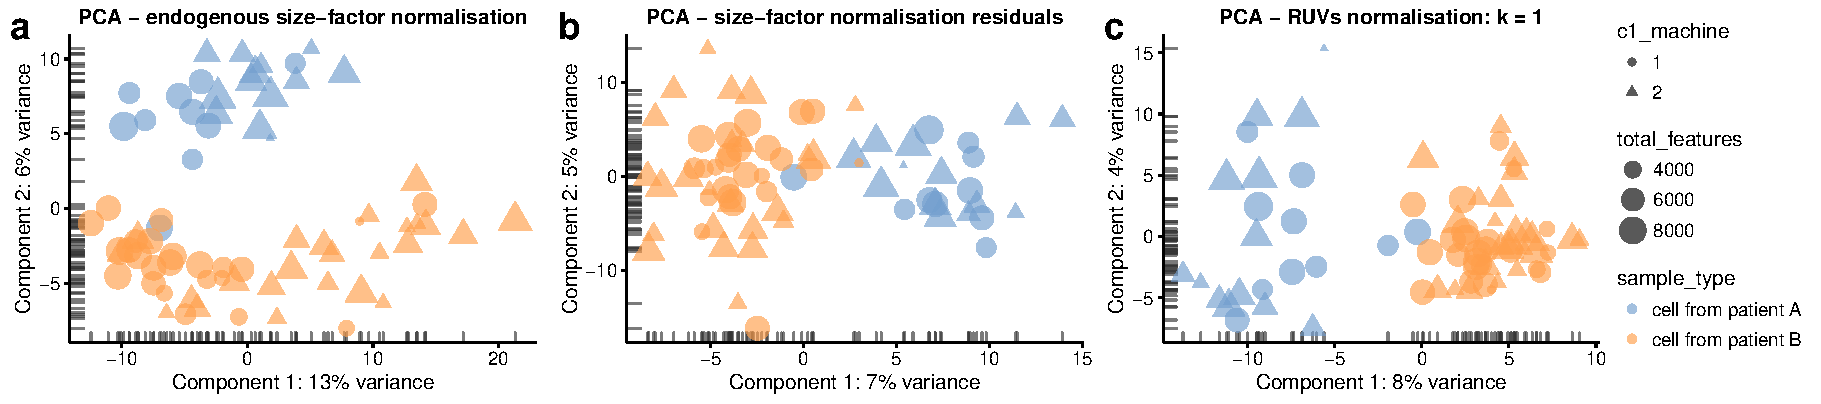
\includegraphics[width=0.48\textwidth]{figures/figure5.pdf}}
\caption{\textbf{Figure 5: Normalisation approaches made easy with
\emph{scater}.} Principal component analysis plots showing cell
structure in the first two PCA dimensions using various normalisation
methods methods that can be easily applied in \emph{scater}, including
endogenous size-factor normalisation using methods from the \emph{scran}
package (\textbf{a}); expression residuals after applying size-factor
normalisation and regressing out known, unwanted sources of variation
(\textbf{b}); and removal of one hidden factor identified using
the RUVs method from the \emph{RUV} package (\textbf{c}). In all plots,
the colour of points is determined by the patient from which cells were
obtained, shape is determined by the C1 machine used to process the
cells and size reflects the total number of genes with detectable
expression in the cell.}\label{fig:05}
\end{figure}

\subsection{Software and data integration}\label{software-and-data-integration}

As part of the R/Bioconductor ecosystem, \emph{scater} can be easily
integrated with other software for scRNA-seq data analysis (Supplementary Figure~2). Because the
SCESet class builds on existing Bioconductor data structures, most
Bioconductor packages for expression analyses are able to operate
seamlessly with SCESet objects. Tools that can integrate easily with
\emph{scater} include many options for data normalisation
\citep{Lun2016-sk,Vallejos2015-ww,Ding2015-jv}, differential expression analysis
\citep{Vallejos2016-qy,Trapnell2014-gj,Finak2015-rd,Vu2016-sk,Kharchenko2014-rx,Korthauer2015-wg,Andrews2016-at}, heterogeneous gene expression analyses
\citep{Lun2016-sk,Vallejos2015-ww}, clustering
\citep{Kiselev2016-fu,Guo2015-wx,Fan2016-wh,Grun2015-fy}, latent or hidden
variable analysis
\citep{Leek2014-nu,Risso2014-np,Stegle2012-is,Chikina2015-lq},
cell cycle phase identification \citep{Scialdone2015-gj} and pseudotime
computation \citep{Trapnell2014-gj,Angerer2015-sw,Julia2015-jt,Campbell2016-es,Campbell2015-nj,Haghverdi2016-is}. The \emph{scater} package bridges
the gap between raw reads and these downstream analysis tools by providing the
pre-processing, QC, visualisation and normalisation methods and a data
structure combining multiple data modalities and metadata necessary for
convenient, robust and reproducible analyses of scRNA-seq data.


\section{Discussion}\label{discussion}

Single-cell RNA sequencing is widely used for high-resolution gene
expression studies investigating the behaviour of individual cells.
While scRNA-seq data can provide substantial biological insights, the
complexity and noise of the data is also much greater than that of
conventional bulk RNA-seq. Thus, rigorous analysis of scRNA-seq data
requires careful quality control to remove low-quality cells and genes,
as well as normalisation to adjust for biases and batch effects in the
expression data. Failure to carry out these procedures correctly is
likely to compromise the validity of all downstream analyses
\citep{Leek2010-nq,Hicks2015-qy,Tung2016-jy,Bacher2016-ay,Grun2015-xi}.

Here, we present an R/Bioconductor package, \emph{scater}, that provides
crucial infrastructure and methods for low-level scRNA-seq data
analysis. The package introduces a data structure tailored to scRNA-seq
data that is compatible with a vast number of existing tools in the
Bioconductor project. The \emph{scater} data structure combines multiple
transformations of the expression data with cell and feature (gene or
transcript) metadata and allows data sets to be easily standardised and
shared. Wrapper functions for the popular RNA-seq quantification methods
\emph{kallisto} and \emph{Salmon} facilitate the processing of raw read
sequences to a SCESet object in R with expression data and accompanying
metadata.

Quality control is a vital preliminary step for scRNA-seq and can be a
time-consuming manual task. We present a tool for automated computation
of QC metrics, novel plotting methods for QC and convenient subsetting
and filtering methods to substantially simplify the process of filtering
out unwanted or problematic cells and genes. The package provides a
large array of sophisticated plotting functions so that cells can be
visualised with a variety of popular dimensionality-reduction techniques
in plots that incorporate cell metadata and expression values as
plotting variables.

Normalisation is a critical aspect of scRNA-seq data processing that is supported by \emph{scater}. Scaling normalisation methods, including the single-cell specific methods in the \emph{scran} package, are seamlessly integrated into a \emph{scater} workflow. Methods for identifying and removing batch effects and other types of unwanted variation are supported both with internal methods and through integration with a multitude of tools available in the R/Bioconductor environment. Once identified, important covariates and latent variables can be flagged for inclusion in downstream statistical models or their effects regressed out of normalised expression values.

Future development will include further extensions to data structures that will enable tight integration of single-cell transcriptomic, genetic and epigenetic data, as well as further refinement of the methods available as the single-cell field matures. Although \emph{scater} has been produced for
scRNA-seq data, its capabilities are well suited for single-cell qPCR data
and bulk RNA-seq data, and will prove useful for supporting analyses of these data types too.

\section{Conclusion}\label{conclusion}

The \emph{scater} package eases the burden for a user tasked with
producing a high-quality single-cell expression dataset for downstream analysis. The intuitive GUI implemented in \emph{scater} provides an easier entry point into rigorous analysis of scRNA-seq data for users without a
computational background, enabling them to process raw reads into high-quality expression data within a single computing environment. Experienced users can take advantage of \emph{scater}'s data structures, wide array of tools, suitability for scripted analyses and seamless integration with many other R/Bioconductor analysis tools. The data structures and methods in
\emph{scater} provide basic infrastructure upon which new scRNA-seq
analysis tools can be developed. We anticipate that \emph{scater} will be a
useful resource for both analysts and software developers in the
single-cell RNA sequencing field.\vspace*{-10pt}


\section*{Acknowledgements}\label{acknowledgements}

We thank Marco Salvetti for provision of the two samples and Zam Cader for processing the samples. We would also like to acknowledge Peter Donnelly and Oliver Stegle for support and helpful discussions.\vspace*{-12pt}

\section*{Funding}

DJM was supported by funding through an Early Career Fellowship from the National Health and Medical Research Council of Australia, and by core funding from EMBL. ATLL was supported by core funding from Cancer Research UK (award no. A17197). KRC is supported by a UK Medical Research Council studentship.\vspace*{-12pt}

\bibliographystyle{natbib}
%\bibliographystyle{achemnat}
%\bibliographystyle{plainnat}
%\bibliographystyle{abbrv}
%\bibliographystyle{plain}
%\bibliographystyle{bioinformatics}
\bibliography{main}


\end{document}
